\documentclass[12pt,onecolumn]{IEEEtran}
\usepackage{graphicx, graphics,epsfig}
\usepackage{color,cite}
\usepackage{amssymb, amsmath}
\usepackage{algorithm}
\usepackage{algorithmic}
\usepackage{url}
\usepackage{amsfonts}
\usepackage{latexsym}
\usepackage{tabularx}
\usepackage{fixltx2e}
%\usepackage{hyphenat}
%\usepackage{underscore}

\newcommand{\ab}{\allowbreak}
%\newcommand{\bus}{\allowbreak\_}
\newcommand{\bus}{\_\allowbreak}
\newcommand{\bas}{/\allowbreak}

\input{../macros/macros}

\title{Group Allocator}
\author{
{
  Sanjeev Mehrotra
}
}

\begin{document}

\maketitle

\section{Introduction}
A generic allocator attempts to match {\em requested resources}, $R$, to
an optimal (in some sense)
{\em allocatable resource location index}, $l_{opt} \in \{0, 1, \dots, L-1\}$
with the location having {\em allocatable resources}, $A_{l_{opt}}$ and
$N_i$ being the name of the $i$th resource location.
$A_l$ are the allocatable resources available at allocatable location index
$l$ and 
$L$ is the number of possible allocatable resource locations.
If no location is found which satisfies the constraints for the requested
resources, it sets $l_{opt}=-1$.
Let $\mathcal{F} \subseteq \{N_0,N_1,\dots,N_{L-1}\}$ be the set of feasible
resource location names, 
and let $s_l$ be a {\em score} at location $l \in \mathcal{F}$.
Then,
\bea
l_{opt} = \left\{
\ba{ll}
\argmax_{j \in \mathcal{F}} s_j & \mbox{if $\mathcal{F} \neq \emptyset$} \\
-1 & \mbox{if $\mathcal{F} = \emptyset$}
\ea
\right.
\eea
For example, in Figure~\ref{fig:req1}, 
the allocator matches the given requested resources, $R$,
to the allocatable resources at location $1$.

We represent the requested resources as $R$, where $R$ is a hash-map,
i.e. a list of $(K,V)$ key-value pairs,
with a key \texttt{request{\bus}name} taken from a set,
\texttt{requested{\bus}resources}.
That is $R[\texttt{request{\bus}name}]$ specifies the value needed
to satisfy the request, with 
$\texttt{request{\bus}name} \in \texttt{requested{\bus}resources}$.
The exact function to used to determine the score and see if an 
allocatable resource location can satisfy the requested resource
is completely arbitrary and can be dependent on the \texttt{request{\bus}name}
or the allocatable resource being used to satisfy the request.

We represent the allocatable resources at location $l$ as
$A_l$, where $A_l$ is a hash-map with a key
\texttt{alloc{\bus}name} taken from a set of available
resources at location $l$, given by \texttt{allocatable{\bus}resources{\bus}l}.

For a location $l$ to satisfy the request, for each requested resource,
$R[\texttt{request{\bus}name}]$, there must be an allocatable resource,
$A_l[\texttt{alloc{\bus}name}]$ which satisfies the request.
Let $M_l$ be this mapping from requested resource to allocatable resource.
That is $M_l[\texttt{request{\bus}name}]$ is a value in the
set \texttt{allocatable{\bus}resources{\bus}l}.
If no allocatable resource specifies the request, then
$M_l[\texttt{request{\bus}name}] = \texttt{nil}$.
Then, we can define the feasible set as the following.
\bea
& \mathcal{F} = \{
N_l | l \in \{0,1,\dots,L-1\}, \nn \\
& \hspace{.2in} M_l[\texttt{request{\bus}name}] \neq \texttt{nil}
& \forall \texttt{request{\bus}name} \in \texttt{requested{\bus}resources}
\}.
\eea
We note that $M_l[\texttt{request{\bus}name}]$ may have constraints, that
is a given requested resource may only be satisfied by certain allocatable
resources.  
For example, a CPU request can only be satisfied by
an allocatable CPU resource, and not for example memory.

\begin{figure*}  
\begin{center}  
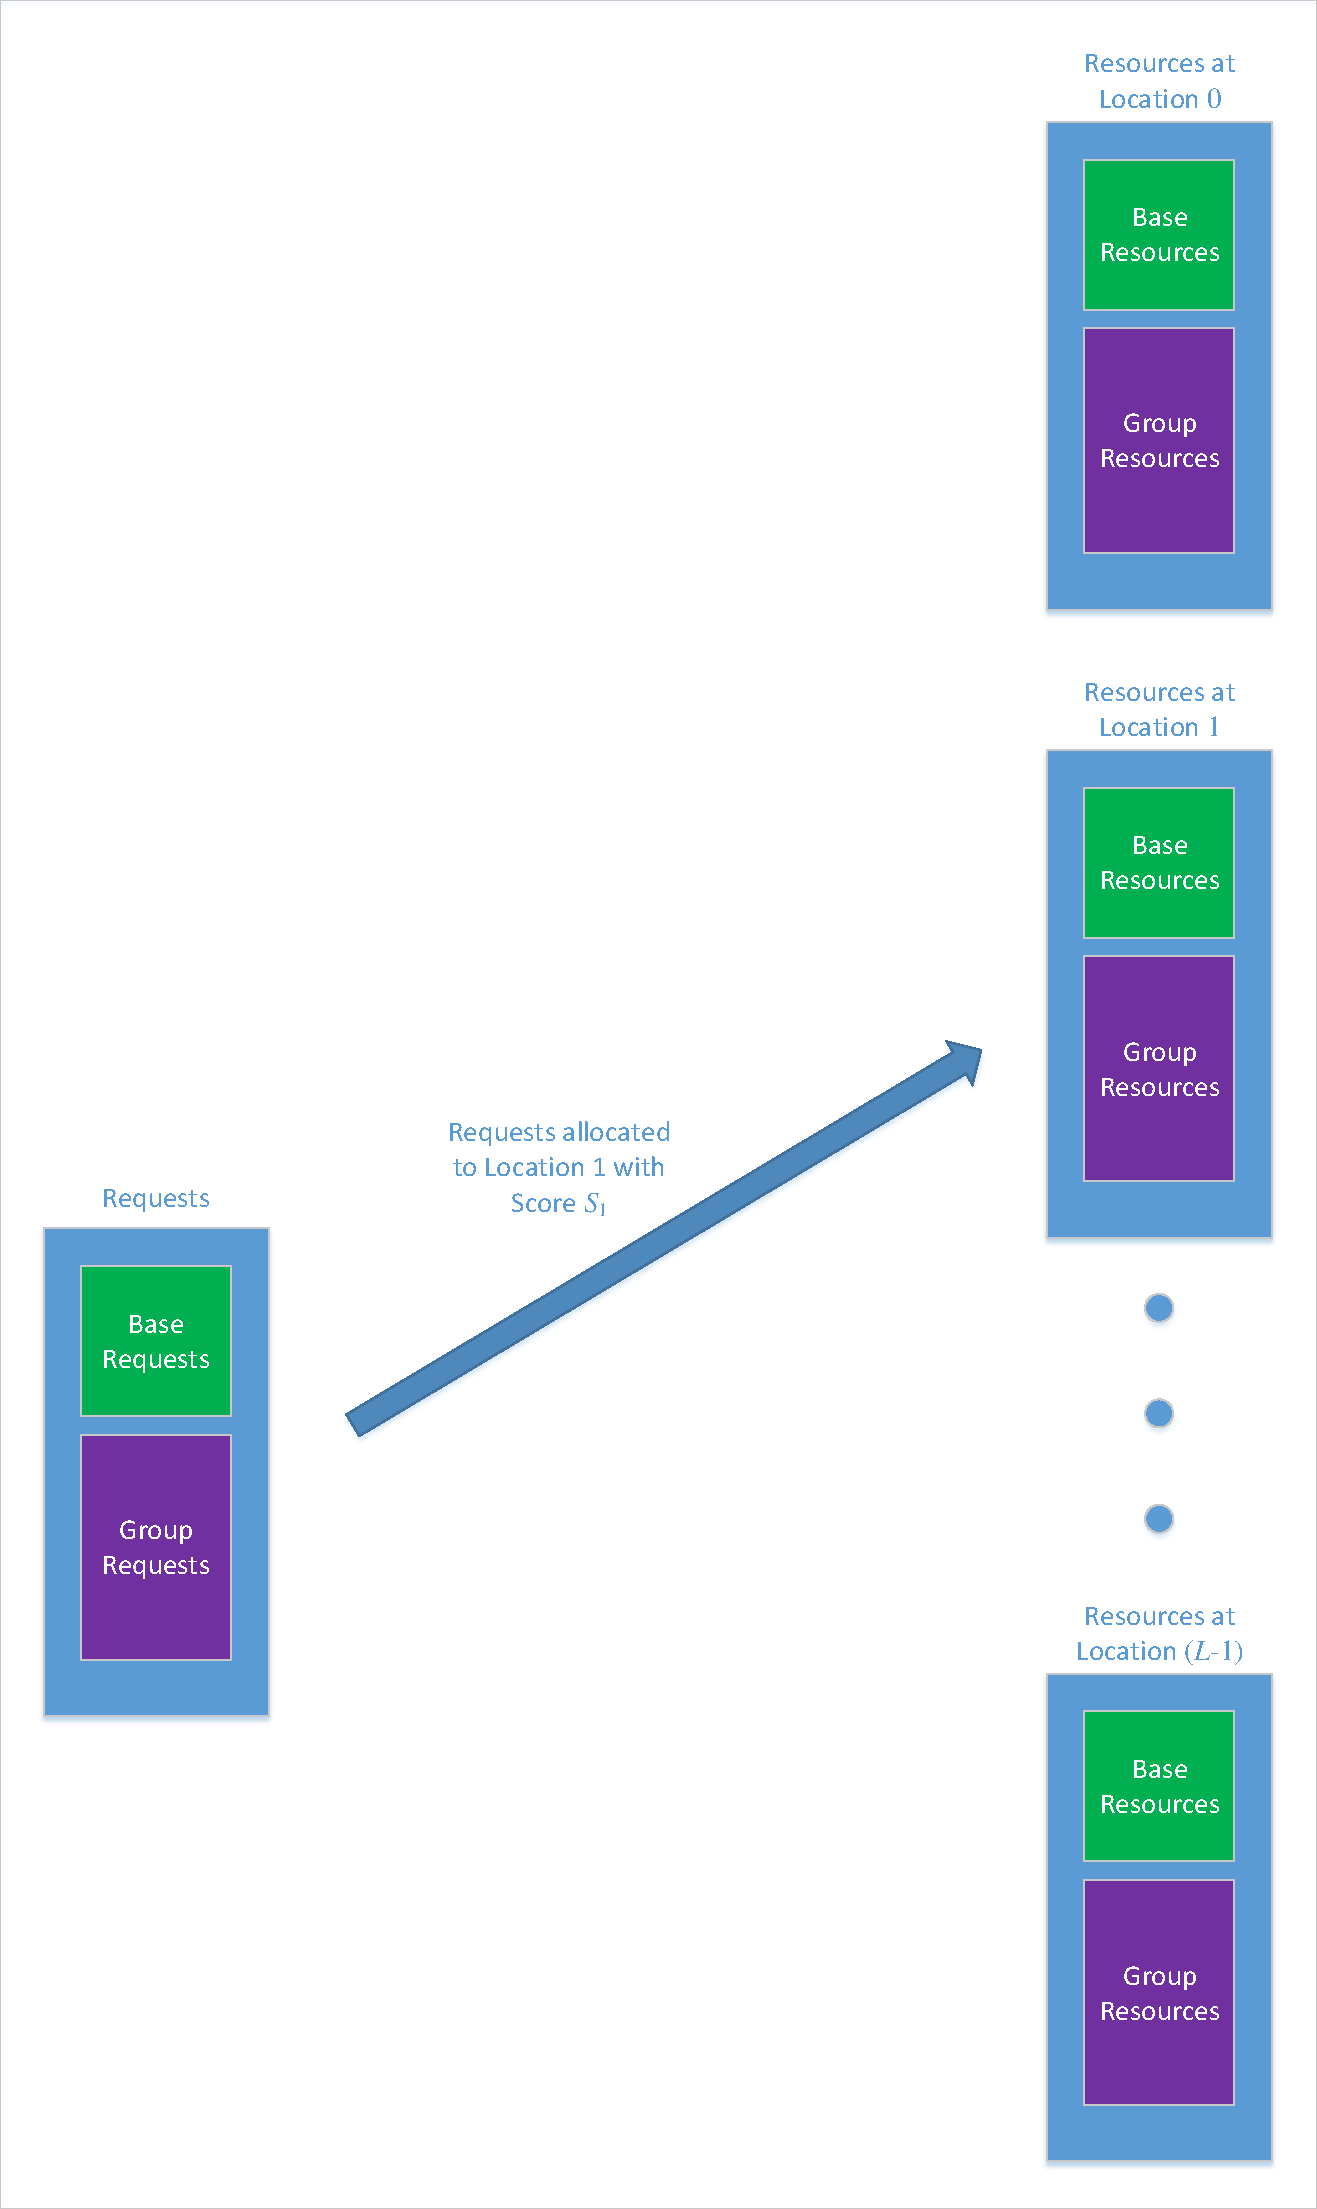
\includegraphics[height=7in,width=6in]{req1.pdf}
\caption{Showing requests mapping to resources at 
given location\label{fig:req1}}
\end{center}  
\end{figure*}  

In the Kubernetes framework, such an allocator can be used to find the
node to schedule a pod on, or can simply be used to see if resources
fit on a given node by giving it one available resource location which
is the node being tested to start with.

\subsection{Example}
\label{sec:example}

As an example, $R$ is the set of requested resources as
in 
\ttfamily
\begin{itemize}
\item[] cpu: 2
\item[] memory: 1GiB.
\end{itemize}
\normalfont
Here the set of 
\texttt{requested{\bus}resources} = $\{\texttt{cpu},\texttt{memory}\}$,
and thus \texttt{resource{\bus}name} can either be \texttt{cpu} or \texttt{memory}.
For simplicity, we write this as
$R=$\texttt{map[cpu: 2 memory: 1GiB]}.

Similarly, $A_l$ is the set of allocatable resources at location $l$.
For example $A_1$ can be the set of allocatable resources at location $1$
given
by 
\ttfamily
\begin{itemize}
\item[] cpu: 4
\item[] memory: 2GiB.
\end{itemize} 
\normalfont
Here \texttt{allocatable{\bus}resources{\bus}1} = $\{\texttt{cpu},\texttt{memory}\}$,
and again \texttt{alloc{\bus}name} can either be \texttt{cpu} or \texttt{memory}.
We can write $A_1=$\texttt{map[cpu: 4 memory: 2GiB]}.

\section{Group allocator}

In the simple case as given in Sec.~\ref{sec:example},
the allocator can compare key by key to see if
the requested resources $R$ can fit onto 
allocatable resources at location $l$, $A_l$. For example compare
requested \texttt{cpu} with allocatable \texttt{cpu} and similarly
for \texttt{memory}.
It does not make sense for a requested CPU resource to be satisfied
by an allocatable memory resource.
Thus, for any $l$, $M_l[\texttt{cpu}] = \texttt{cpu}$ if sufficient
CPU is available, otherwise $M_l[\texttt{cpu}]=\texttt{nil}$.
The same is true for memory.
Having only such resources makes the job of the allocator
fairly straightforward.
Thus for simple cases like this, the mapping, $M_l$ is not something
that is found by the allocator, but rather a static identity map.

However, this becomes infeasible for more complicated scenarios.
As an example, consider GPU resources, where a single location
can have multiple GPUs, each with differing memory
and similarly, the request can require a number of GPUs with
differing memory requirements.
Although it may seem difficult to express such constraints with simple
key-value pairs for the requested resources and allocatable resources,
it is fairly doable.
For example, one way to do this is to express requested resources and
allocatable resources for each GPU {\em separately}.
Then, we can write requested resources, $R$, as
\ttfamily
\begin{itemize}
\item[] cpu: 2
\item[] memory: 1GiB
\item[] gpu/0/cards: 1
\item[] gpu/0/memory: 1GiB
\item[] gpu/1/cards: 1
\item[] gpu/1/memory: 2GiB,
\end{itemize}
\normalfont
where 
we have requested 1 GPU with minimum 1GiB memory and another with
minimum 2GiB memory.

Similarly, a resource location can advertise allocatable resources, $A_l$, as
\ttfamily
\begin{itemize}
\item[] cpu: 4
\item[] memory: 2GiB
\item[] gpu/dev0/cards: 1
\item[] gpu/dev0/memory: 1GiB
\item[] gpu/dev1/cards: 1
\item[] gpu/dev1/memory: 3GiB
\item[] gpu/dev2/cards: 1
\item[] gpu/dev2/memory: 2GiB
\item[] gpu/dev3/cards: 1
\item[] gpu/dev3/memory: 4GiB,
\end{itemize}
\normalfont
where we have 4 GPUs with differing memory on the node.

In such a case, a simple allocator cannot just look for a resource with
the same key as that being requested.
For example, it is clear that the request can be satisfied by
the resource location.
However, there is no key \texttt{gpu/0/cards} present in the resource
location even though it is a requested key.
This is the main need for what we define as the {\em group allocator}.

The job of the group allocator becomes the following.
\begin{itemize}
\item 
Find the best allocatable resource location index(in some sense), $l_{opt}$,
amongst the feasible set, $\mathcal{F}$.
\item 
Obtain the mapping from requested resource to allocatable resource
on for that best allocatable resource location, $M_{l_{opt}}$.
\end{itemize}
In the process of determining $l_{opt}$, the allocator may compute
a score for each location to find the best one.

The second item is needed as the map will not be the identity map anymore.
An example of such a mapping, $M_{l_{opt}}$, could be the following.
\texttt{
\begin{itemize}
\item[] cpu: cpu
\item[] memory: memory
\item[] gpu/0/cards: gpu/dev0/cards
\item[] gpu/0/memory: gpu/dev0/memory
\item[] gpu/1/cards: gpu/dev2/cards
\item[] gpu/1/memory: gpu/dev2/memory
\end{itemize}
}

\subsection{Partitioning}

The first task of the group allocator is partitioning.
Both the requested resources as well as the allocatable resources 
of a given location are partitioned into ``base'' and ``group'' resources.
A base resource is one which can directly be compared
by looking at the key.
For example, a base requested resource requires a base allocatable resource
with the same key, for example, in the example above \texttt{cpu} and
\texttt{memory}.
That is for a base resource
\bea
M_l[\texttt{request{\bus}name}] = \texttt{request{\bus}name}.
\eea
A ``group'' resource on the other hand, may match a requested
resource to an allocatable resource with a differing key.

In our framework,
all requested resources which are of the format,
\bea
\texttt{request{\bus}name} =
\texttt{request{\bus}groupname\slash request{\bus}groupindex\slash request{\bus}basename}
\eea
are considered to be ``group'' requested resources by the allocator, where
the keys are in the sets,
\bea
\texttt{request{\bus}groupname} & \in & \texttt{request{\bus}subgroupnames} \\
\texttt{request{\bus}groupindex} & \in & \texttt{request{\bus}subgroupindices[request{\bus}groupname]} \\
\texttt{request{\bus}basename} & \in & \mbox{\footnotesize{\texttt{request{\bus}resourcebasenames[request{\bus}groupname][request{\bus}groupindex]}}}.
\eea

Similarly, all allocatable resource which are of the format,
\bea
\texttt{alloc{\bus}name} =
\texttt{alloc{\bus}groupname/alloc{\bus}groupindex/alloc{\bus}basename}
\eea
are ``group'' allocatable resources, with the keys in the sets
\bea
\texttt{alloc{\bus}groupname} & \in & \texttt{alloc{\bus}subgroupnames} \\
\texttt{alloc{\bus}groupindex} & \in & \texttt{alloc{\bus}subgroupindices[alloc{\bus}groupname]} \\
\texttt{alloc{\bus}basename} & \in & \mbox{\small{\texttt{alloc{\bus}resourcebasenames[alloc{\bus}groupname][alloc{\bus}groupindex]}}}.
\eea

Since for base resources, 
$M_l[\texttt{request{\bus}name}] = \texttt{request{\bus}name}$,
it is sufficient to look at $A_l[$\texttt{req\-uest{\bus}name}$]$
and compare.
If \texttt{request{\bus}name} does not exist in the set
of \texttt{allocatable{\bus}resources}, then the resource request cannot be
satisfied.

To check if a group resource being requested can fit onto a location
with allocatable resources, group resources are first
organized into subgroups.
A new subgroup is formed for each unique combination
of $(\texttt{request{\bus}groupname, request{\bus}groupindex})$,
as
\bea
& R_G[\texttt{request{\bus}groupname}][\texttt{request{\bus}groupindex}]
[\texttt{request{\bus}basename}] = \nn \\
& \hspace{.2in} R[\texttt{request{\bus}groupname}\slash \texttt{request{\bus}groupindex} \slash
\texttt{request{\bus}basename}].
\eea
Similarly, the group allocatable resources at location $l$
which are of the format 
$A_l$\ab[\texttt{alloc{\bus}groupname}]\ab[\texttt{alloc{\bus}groupindex}]
\ab[\texttt{alloc{\bus}basename}]
are partitioned, resulting in a new subgroup for each combination
of $(\texttt{alloc{\bus}groupname, alloc{\bus}groupindex})$,
\bea
& A_{lG}[\texttt{all\-oc{\bus}group\-name}][\texttt{all\-oc{\bus}group\-index}]
[\texttt{alloc{\bus}base\-name}] = \nn \\
& \hspace{.4in} A_l[\texttt{request{\bus}groupname}/\texttt{request{\bus}groupindex}/
\texttt{request{\bus}basename}].
\eea

\subsubsection{Example}

For example, in the example above, the requested resources
produces two requested 
subgroups $R_G[$\texttt{gpu}$][0]$ and $R_G[$\texttt{gpu}$][1]$,
where $R_G[$\texttt{gpu}$][0]$ is given by
\ttfamily
\begin{itemize}
\item[] cards: 1
\item[] memory: 1GiB,
\end{itemize}
\normalfont
and $R_G[$\texttt{gpu}$][1]$ is given by
\ttfamily
\begin{itemize}
\item[] cards: 1
\item[] memory: 2GiB.
\end{itemize}
\normalfont

Similarly, the allocatable resources at the location $1$ produce
four allocatable subgroups, $A_{1G}$\ab[\texttt{gpu}]\ab[\texttt{dev0}], given by
\ttfamily
\begin{itemize}
\item[] cards: 1
\item[] memory: 1GiB,
\end{itemize}
\normalfont
$A_{1G}[\texttt{gpu}][\texttt{dev1}]$ given by,
\ttfamily
\begin{itemize}
\item[] cards: 1
\item[] memory: 2GiB,
\end{itemize}
\normalfont
$A_{1G}[\texttt{gpu}][\texttt{dev2}]$, given by
\ttfamily
\begin{itemize}
\item[] cards: 1
\item[] memory: 2GiB,
\end{itemize}
\normalfont
and $A_{1G}[\texttt{gpu}][\texttt{dev3}]$, given by
\ttfamily
\begin{itemize}
\item[] cards: 1
\item[] memory: 4GiB.
\end{itemize}
\normalfont

\subsection{Allocation}

Now, the group allocator is recursively run on each of the requested
subgroups,
$R_G[$\texttt{req\-uest{\bus}group\-name}$][$\texttt{req\-uest{\bus}group\-index}$]$.
For each requested subgroup, all allocatable subgroups where
\texttt{alloc{\bus}group\-name} = \texttt{request{\bus}group\-name} are
considered as possible resource locations.
The number of possible resource locations for 
the allocation of a subgroup onto resource location $l$ is given by
\bea
L_{lG}[\texttt{request{\bus}groupname}] = 
  \mbox{length}(A_{lG}[\texttt{request{\bus}groupname}]).
\eea
That is it is from the
set \texttt{alloc{\bus}subgroupindices[request{\bus}groupname]}.
Let's call this location 
$n_{lG,opt}[$\texttt{req\-uest{\bus}group\-name}$]
  [$\texttt{req\-uest{\bus}group\-index}$]$.
For simplicity, we can simply denote it as $n_{lG,opt}$.

In addition, the recursive call to the allocator
returns the mapping for the subgroups $M_{lG}$.
The mapping returned by the recursive call to the group allocator for 
the subgroups can be used to get back the mapping for the group 
via the following,
\bea
M_l[\texttt{request{\bus}groupname/request{\bus}groupindex/request{\bus}basename}] 
  = \nn \\
\hspace{.2in}
 \texttt{request{\bus}groupname}/ \nn \\
  \texttt{alloc{\bus}subgroupindices}[n_{lG,opt}]/ \nn \\
 M_{lG}[\texttt{request{\bus}groupname}][\texttt{request{\bus}groupindex}]
    [\texttt{request{\bus}basename}]
\label{eqn:mapp}
\eea
If any of the subgroup allocations fail at location $l$ (i.e., there
is no feasible location for the subgroup), then the 
requested resources cannot fit at location $l$.

If all the subgroup allocation succeed, and if the base resource
allocations are deemed to be sufficient, then a score for location $l$
can be computed to be used by the allocator.

\subsubsection{Example}

For example, when considering the fit for location $1$ using the 
allocatable resource $A_1$, for request $R$,
the group allocator does the following.
\begin{itemize}
\item
Compare the base resources \texttt{cpu} and \texttt{memory} to see if they
fit.
\item
Recursively call the group allocator to see if
$R_G[\texttt{gpu}][0]$ can fit onto any of the allocatable resources
subgroups,
$\{A_{1G}[\texttt{gpu}][\texttt{dev0}], A_{1G}[\texttt{gpu}][\texttt{dev1}],
A_{1G}[\texttt{gpu}][\texttt{dev2}], A_{1G}[\texttt{gpu}][\texttt{dev3}]\}$.
The group allocator returns $(fit, mapping)$.
Let $M_{1G}[\texttt{gpu}][0]$ be the mapping and
let $n_{1G}[\texttt{gpu}][0] \in \{-1, 0,1,2,3\}$ be the optimal location index.
-1 specifies that no location was found out of the four locations.
\item
Recursively call the group allocator to see if
$R_G[\texttt{gpu}][1]$ can fit onto any of the allocatable resources
subgroups,
$\{A_{1G}[\texttt{gpu}][\texttt{dev0}], A_{1G}[\texttt{gpu}][\texttt{dev1}],
A_{1G}[\texttt{gpu}][\texttt{dev2}], A_{1G}[\texttt{gpu}][\texttt{dev3}]\}$.
The group allocator returns $(fit, mapping)$.
Let $M_{1G}[\texttt{gpu}][1]$ be the mapping and
let $n_{1G}[\texttt{gpu}][1] \in \{-1, 0,1,2,3\}$ be the optimal location index.
-1 specifies that no location was found out of the four locations.
\item
If the base resources fit, and the recursive calls to the group
allocator return a fit (i.e. a location not equal to $-1$),
then the requested resources can fit.
\item
From Eqn.~\ref{eqn:mapp}, obtain the final mapping using the following.
\ttfamily
\begin{itemize}
\item[] cpu: cpu
\item[] memory: memory
\item[] gpu/0/cards: gpu/alloc{\bus}subgroupindices[$n_{1G,opt}$[gpu][0]]/cards
\item[] gpu/0/memory: gpu/alloc{\bus}subgroupindices[$n_{1G,opt}$[gpu][0]]/memory
\item[] gpu/1/cards: gpu/alloc{\bus}subgroupindices[$n_{1G,opt}$[gpu][1]]/cards
\item[] gpu/1/memory: gpu/alloc{\bus}subgroupindices[$n_{1G,opt}$[gpu][1]]/memory,
\end{itemize}
\normalfont
where $n_{1G,opt}[\texttt{gpu}][\texttt{request{\bus}groupindex}]$ 
is the location of the allocatable
subgroup with \texttt{alloc{\bus}name=gpu} returned
by the recursive call to the group allocator.
Note that 
\texttt{alloc{\bus}sub\-group\-indices[$n_{1G,opt}$[gpu][*]]} will be from
the set $\{\texttt{dev0, dev1, dev2, dev3}\}$.
\item
If a fit is found, then a score is computed for location $1$.
\end{itemize}

For example, suppose $n_{1G,opt}[\texttt{gpu}][0]=0$ 
and $n_{1G,opt}[\texttt{gpu}][1]=2$,
then \texttt{alloc{\bus}sub\-group\-indices\allowbreak[$n_{1G,opt}$[gpu][0]] \allowbreak= \allowbreak dev0}
and \texttt{alloc{\bus}sub\-group\-indices[$n_{1G,opt}$[gpu][1]] = dev2}.
The recursive call to the group allocator returns
the mapping for both subgroups, as $M_{1G}$\ab[\texttt{gpu}]\ab[$0$] and
$M_{1G}$\ab[\texttt{gpu}]\ab[$1$], which are both given by,
\ttfamily
\begin{itemize}
\item[] cards : cards
\item[] memory : memory.
\end{itemize}
\normalfont
Then, using Eqn.~\ref{eqn:mapp}, we get the following mapping
\ttfamily
\begin{itemize}
\item[] cpu: cpu
\item[] memory: memory
\item[] gpu/0/cards: gpu/dev0/cards
\item[] gpu/0/memory: gpu/dev0/memory
\item[] gpu/1/cards: gpu/dev2/cards
\item[] gpu/1/memory: gpu/dev2/memory,
\end{itemize}
\normalfont

In the final mapping, for base resources,
$M[\texttt{resource}] = \texttt{resource}$.
For group resources, 
the \texttt{request{\bus}groupindex} for the requested resource
is replaced by
\texttt{alloc{\bus}sub\-group\-indices[$n_{1G,opt}$\ab[req\-uest{\bus}group\-name]\ab[req\-uest{\bus}group\-index]]}, 
where $n_{1G,opt}$ is the best location for the subgroup
amongst the allocatable subgroups with the same groupname.

\subsection{Scorer}
\label{sec:score}

One component which can be used to find the best location
amongst a list of allocatable resource locations is a scorer.
For a location $l$,
it uses allocatable resources, $A_l$, and resources already being used
along with the requested resources, $R$, and requested resource mapping $M$
to find a score for the fit.
We define $s_l$ to be the score for the location $l$.
Let $U_l$ be the resources being used at location $l$.
It is a hash-map with the same keys used to index $A_l$, that is
it is indexed using \texttt{alloc{\bus}name}.

We define $s_l$ to be the sum of scores over all allocatable resources,
that is
\bea
& RL_l[\texttt{alloc{\bus}name}] = \{R[\texttt{request{\bus}name}]: M_l[\texttt{request{\bus}name}]=\texttt{alloc{\bus}name}\} \label{eqn:rlist} \\
& s_l = \sum\limits_{\texttt{alloc{\bus}name} \in \texttt{allocatable{\bus}resources{\bus}l}} 
  S_{\texttt{alloc{\bus}name}}
\parbox[t]{3in}{
$(A_l[\texttt{alloc{\bus}name}]$, \\
$U_l[\texttt{alloc{\bus}name}]$, \\
$RL_l[\texttt{alloc{\bus}name}])$
}
\label{eqn:scorel}
\eea
that is the scorer function $S_{\texttt{alloc{\bus}name}}$ itself is a function
of the resource being allocated upon, and it is a function
of the allocatable resource $A_l$ for the given resource,
the amount of used resource $U_l$ for the given resource, and
the list of requests $R$ which map to using the given resource.
In addition to a score, the scorer can also tell whether a
sufficient amount of allocatable resource exists in order to satisfy
the request.
For example, the scorer could return -1 to denote that sufficient resource
does not exist.
In practice, the first step the scorer will do is 
find a list of resources being mapped to a given allocatable resource, $RL$,
as in Eqn.~\ref{eqn:rlist}.
The list $RL$ is then passed to the scorer.

In addition to computing the score, an arbitrary function,
$\Phi_{\texttt{alloc{\bus}name}}$, can be
used to update the used resources for an allocatable resource,
$U_l[\texttt{alloc{\bus}name}]$, using
\bea
U'_l[\texttt{alloc{\bus}name}] = 
  \Phi_{\texttt{alloc{\bus}name}}(A_l[\texttt{alloc{\bus}name}], U_l[\texttt{alloc{\bus}name}],
       RL_l[\texttt{alloc{\bus}name}]),
\eea
where $U'_l$ is used to denote the updated used resources.

Note that the scorer function, $S$, and used resource updater, $\Phi$,
can also be dependent upon the request
being made, and can also have additional state that may be needed.
As an example, in Kubernetes, pods consist of
both initialization containers and running containers.
Initialization containers are first run sequentially (one-by-one),
and once all initialization containers complete, then all running
containers are run in parallel.
Here, the scorer itself is dependent upon whether the request is
being made on behalf of a running container or an initialization container.
In addition, additional state such as the resource being requested
by the pod can be used as additional state for the scorer.
Thus in an actual implementation of the scorer function, additional
parameters may be passed in.

As an example, for linearly consumable resources, we can use the
following for the resource updater and scorer.
The resource updater and scorer must run in a particular
order.
When resources are being consumed, all running containers must be
updated and scored first, followed by initialization containers.
Let $P[\texttt{alloc{\bus}name}]$ be the resources being consumed by a pod.
Then, we first run the following for running containers.
\bea
P'_l[\texttt{alloc{\bus}name}] &=& P_l[\texttt{alloc{\bus}name}] + RL_l[\texttt{alloc{\bus}name}] \\
U'_l[\texttt{alloc{\bus}name}] &=& U_l[\texttt{alloc{\bus}name}] + RL_l[\texttt{alloc{\bus}name}] \\
s_l &=& \frac{U'_l[\texttt{alloc{\bus}name}]}{A_l[\texttt{alloc{\bus}name}]}
\eea
Then, for initialization containers, we do the following
\bea
P'_l[\texttt{alloc{\bus}name}] &=& \max(P_l[\texttt{alloc{\bus}name}], RL_l[\texttt{alloc{\bus}name}]) \\
U'_l[\texttt{alloc{\bus}name}] &=& U_l[\texttt{alloc{\bus}name}] + 
  (P'_l[\texttt{alloc{\bus}name}]-P_l[\texttt{alloc{\bus}name}]) \\
s_l &=& \frac{U'_l[\texttt{alloc{\bus}name}]}{A_l[\texttt{alloc{\bus}name}]}
\eea
We see that for initialization containers, additional state regarding
the amount of resources being used by running containers for the pod
is used as an additional variable to modify the function $\Phi$.
If we put all equations together, we get the following for the scorer,
\bea
s_l &=& \frac{U_l[\texttt{alloc{\bus}name}] + \max(P_l[\texttt{alloc{\bus}name}], RL_l[\texttt{alloc{\bus}name}]) - P_l[\texttt{alloc{\bus}name}]}{A_l[\texttt{alloc{\bus}name}]},
\eea
and thus it is also a function of current pod usage.

When a pod is being removed from a node, then
the entire pod usage is first computed and then subtracted
from the node usage.

\section{Implementation in Kubernetes}

\sloppy
The group allocator is implemented in Kubernetes in the file
\texttt{plugin{\bas}pkg{\bas}scheduler{\bas}algorithm{\bas}
   predicates{\bas}grpallocate.go}.
All requested resources as well as allocatable resources on a node
with the prefix
\texttt{alpha.kubernetes.io{\bas}group-resource} are considered
to be ``group'' resources.
The type \texttt{GrpAllocator} is the main class which performs
the group allocator and stores state.

The group allocator's job is two-fold, one to find a suitable
location for the requested resources amongst the {\em resource locations}
with {\em allocatable resources} and two to find a mapping between
requested resources and allocatable resources on the resource location.

Initially, we consider there to be only one resource location,
which is the node group resources.
So the initial group allocator call attempts to find whether
the node is able to satisfy the requests and if it can satisfy the
requests, then it also outputs a mapping between requests and allocatable
resources on the node.

The variables \texttt{RequiredResource} and \texttt{AllocResource}
correspond to key-value pairs with keys being strings and value being
int64 corresponding to the required and allocatable resources at a given node
respectively.
These correspond to resources at the top-level group allocator.

The actual required resource and allocatable resource for a given group
are specified in
\texttt{GrpRequiredResource} and \texttt{GrpAllocResource} which 
are string to string mappings.
Therefore, 
\texttt{GrpRequiredResource map[string]string}
is a map whose keys specify the names of the requested resources.
And, \texttt{RequiredResources[GrpRequiredResource[resource{\bus}key]]} is the
amount of requested resource for with the name \texttt{resource{\bus}key}.
In addition, \texttt{GrpAllocResource map[string](map[string]string)}
is a map whose keys specify locations for resource locations.
And, \texttt{GrpAllocResource[resource{\bus}location{\bus}key]} specifies a list
whose keys specify the resources available at the allocatable location
\texttt{resource{\bus}location{\bus}key}.
And 
\texttt{AllocResource[GrpAllocResource[resource{\bus}location{\bus}key][resource{\bus}key]]}
specifies the amount of allocatable resource at resource location
\texttt{resource{\bus}location{\bus}key} with the name \texttt{resource{\bus}key}.

For simplicity all variables in the group allocator are specified with
respect to the top level group.
The actual ones for a given group are simply found
by first looking up in
\texttt{GrpRequiredResource} or \texttt{GrpAllocResource} to find
the actual key for a given group.

The group allocator consists of several core functions.
\begin{itemize}
\item
\texttt{allocateGroup} allocates requested resources
amongst a list of resource locations.
It then picks a location with the best score amongst the list
of feasible locations, provided one exists.
\item
\texttt{allocateGroupAt} attempts to allocate the request to a particular
location and if it fits, it finds a score, along with a requested
resource to allocatable resource mapping.
\item
\texttt{resourceAvailable} checks if sufficient {\em base resources}
are available at the resource location.
\item
\texttt{allocateSubGroups} performs recursive calls to allocateGroup
for all subgroups, if any exist.
\item
\texttt{findScoreAndUpdate} performs scoring for the allocation and
updates used resources.
\end{itemize}

The scorer is a function with signature, \\
\texttt{
func(allocatableResource int64, usedByPod int64, usedByNode int64, requested []int64, initContainer bool) (found bool, score float64, usedByContainer int64, newUsedByPod, newUsedByNode int64)
} \\
It is specified for all allocatable resources at a given node.
A different function may be used to determine fit if desired.

\section{GPU Affinity Example}

Here we provide an example of using the group allocator for
allocating GPUs with affinity.
GPUs are often connected via a high speed peer-to-peer link, for example,
NVLink in NVIDIA GPUs with Pascal architecture as shown
in Fig.~\ref{fig:gpu}. GPU0 is connected via high-speed interconnect
to GPU1 and a lower speed interconnect to GPU2 and GPU3.

\begin{figure*}  
\begin{center}  
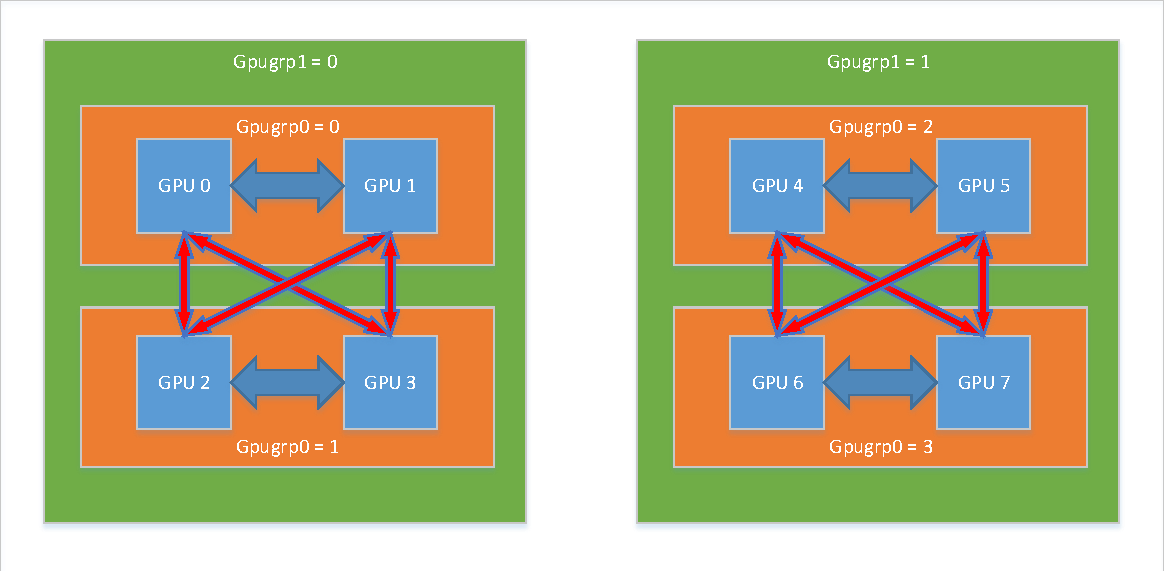
\includegraphics[width=6in]{gpu.pdf}
\caption{GPU with NVLink and corresponding GPU groups, showing
both high speed and lower speed interconnects.\label{fig:gpu}}
\end{center}  
\end{figure*}

Then, one way to specify allocatable resources is the following.
\ttfamily
\begin{itemize}
\item[] Gpugrp1/0/Gpugrp0/0/gpu/dev0/cards: 1
\item[] Gpugrp1/0/Gpugrp0/0/gpu/dev1/cards: 1
\item[] Gpugrp1/0/Gpugrp0/1/gpu/dev2/cards: 1
\item[] Gpugrp1/0/Gpugrp0/1/gpu/dev3/cards: 1
\item[] Gpugrp1/1/Gpugrp0/2/gpu/dev4/cards: 1
\item[] Gpugrp1/1/Gpugrp0/2/gpu/dev5/cards: 1
\item[] Gpugrp1/1/Gpugrp0/3/gpu/dev6/cards: 1
\item[] Gpugrp1/1/Gpugrp0/3/gpu/dev7/cards: 1
\end{itemize}
\normalfont
That is, two GPUs with high-speed interconnect 
are first grouped into Gpugrp0, with indices $\{0,1,2,3\}$.
Then, two successive groups of Gpugrp0 are grouped into Gpugrp1
which has the lower speed interconnect, with indices $\{0, 1\}$.

Requested resources can be similarly grouped depending on
which interconnects are required.
For example,
\ttfamily
\begin{itemize}
\item[] Gpugrp1/R0/Gpugrp0/RA/gpu/gpu0/cards: 1
\item[] Gpugrp1/R0/Gpugrp0/RA/gpu/gpu1/cards: 1
\item[] Gpugrp1/R1/Gpugrp0/RA/gpu/gpu2/cards: 1
\item[] Gpugrp1/R1/Gpugrp0/RA/gpu/gpu3/cards: 1
\item[] Gpugrp1/R1/Gpugrp0/RB/gpu/gpu4/cards: 1
\item[] Gpugrp1/R1/Gpugrp0/RB/gpu/gpu5/cards: 1
\end{itemize}
\normalfont
The top-level group allocator will make two recursive
calls to group allocate \texttt{request{\bus}groupname = Gpugrp1} with
\texttt{request{\bus}groupindex = 0} and
\texttt{request{\bus}groupindex = 1}.

The call to allocate \texttt{request{\bus}groupname = Gpugrp1} for
\texttt{request{\bus}groupindex = 0} will then
make a single recursive call to group allocate
\texttt{request{\bus}groupname = Gpugrp0} with
\texttt{request{\bus}groupindex = A}.
This in turn will make two recursive calls to group allocate
\texttt{request{\bus}groupname = gpu} with 
\texttt{request{\bus}groupindex = dev0} and another
for 
\texttt{request{\bus}groupname = gpu} with 
\texttt{request{\bus}groupindex = dev1}.
Each of these will have the base resource of \texttt{cards}.

The call to allocate \texttt{request{\bus}groupname = Gpugrp1} for
\texttt{request{\bus}groupindex = 1} will then
make two recursive call to group allocate, one for
\texttt{request{\bus}groupname = Gpugrp0} with
\texttt{request{\bus}groupindex = A} and another for
\texttt{request{\bus}groupname = Gpugrp0} with
\texttt{request{\bus}groupindex = B}.
Each of these two will make two more recursive calls.

The final allocations to perform will be the following.
\ttfamily
\begin{verbatim}
<TopLevel>
  Gpugrp1/R0
    Gpugrp1/R0/Gpugrp0/RA
      Gpugrp1/R0/Gpugrp0/RA/gpu/gpu0
        Gpugrp1/R0/Gpugrp0/RA/gpu/gpu0/cards -- base resource
      Gpugrp1/R0/Gpugrp0/RA/gpu/gpu1
        Gpugrp1/R0/Gpugrp0/RA/gpu/gpu1/cards -- base resource
  Gpugrp1/R1
    Gpugrp1/R1/Gpugrp0/RA
      Gpugrp1/R1/Gpugrp0/RA/gpu/gpu2
        Gpugrp1/R1/Gpugrp0/RA/gpu/gpu2/cards -- base resource
      Gpugrp1/R1/Gpugrp0/RA/gpu/gpu3
        Gpugrp1/R1/Gpugrp0/RA/gpu/gpu3/cards -- base resource
    Gpugrp1/R1/Gpugrp0/RB
      Gpugrp1/R1/Gpugrp0/RB/gpu/gpu4
        Gpugrp1/R1/Gpugrp0/RB/gpu/gpu4/cards -- base resource
      Gpugrp1/R1/Gpugrp0/RB/gpu/gpu5
        Gpugrp1/R1/Gpugrp0/RB/gpu/gpu5/cards -- base resource
\end{verbatim}
\normalfont

Of course, each allocation will attempt to search for multiple locations
for the fit.
A diagram showing the call is shown in Fig.~\ref{fig:alloc}.
The green circles show group allocators. 
The blue boxes show the allocatable locations being searched.
Each blue box will perform a search for all resources which 
are considered as ``base resources'' for that level.
Each blue box may have further subgroups to search which will
be shown as descendants of the blue box.
If there are no group resources left (i.e. all resources are base
resources), then the box will have no descendants.
For example, the leaf of the tree at the top right of the figure is
requested subgroup \texttt{Grp1/R0/Grp0/RA/gpu/0} checking
if resources fit onto \texttt{Grp1/0/Grp0/0/gpu/dev0}.
The only requested resource is \texttt{cards} which is checked.
Each group allocator (green circle) picks the best of all locations.
That is it picks the best blue box which descends from the node.
In the figure, for simplicity, only the \texttt{Grp1/R0} branch is shown.
Another branch for \texttt{Grp1/R1} will also be present which is not
shown in the figure.

\begin{figure*}  
\begin{center}  
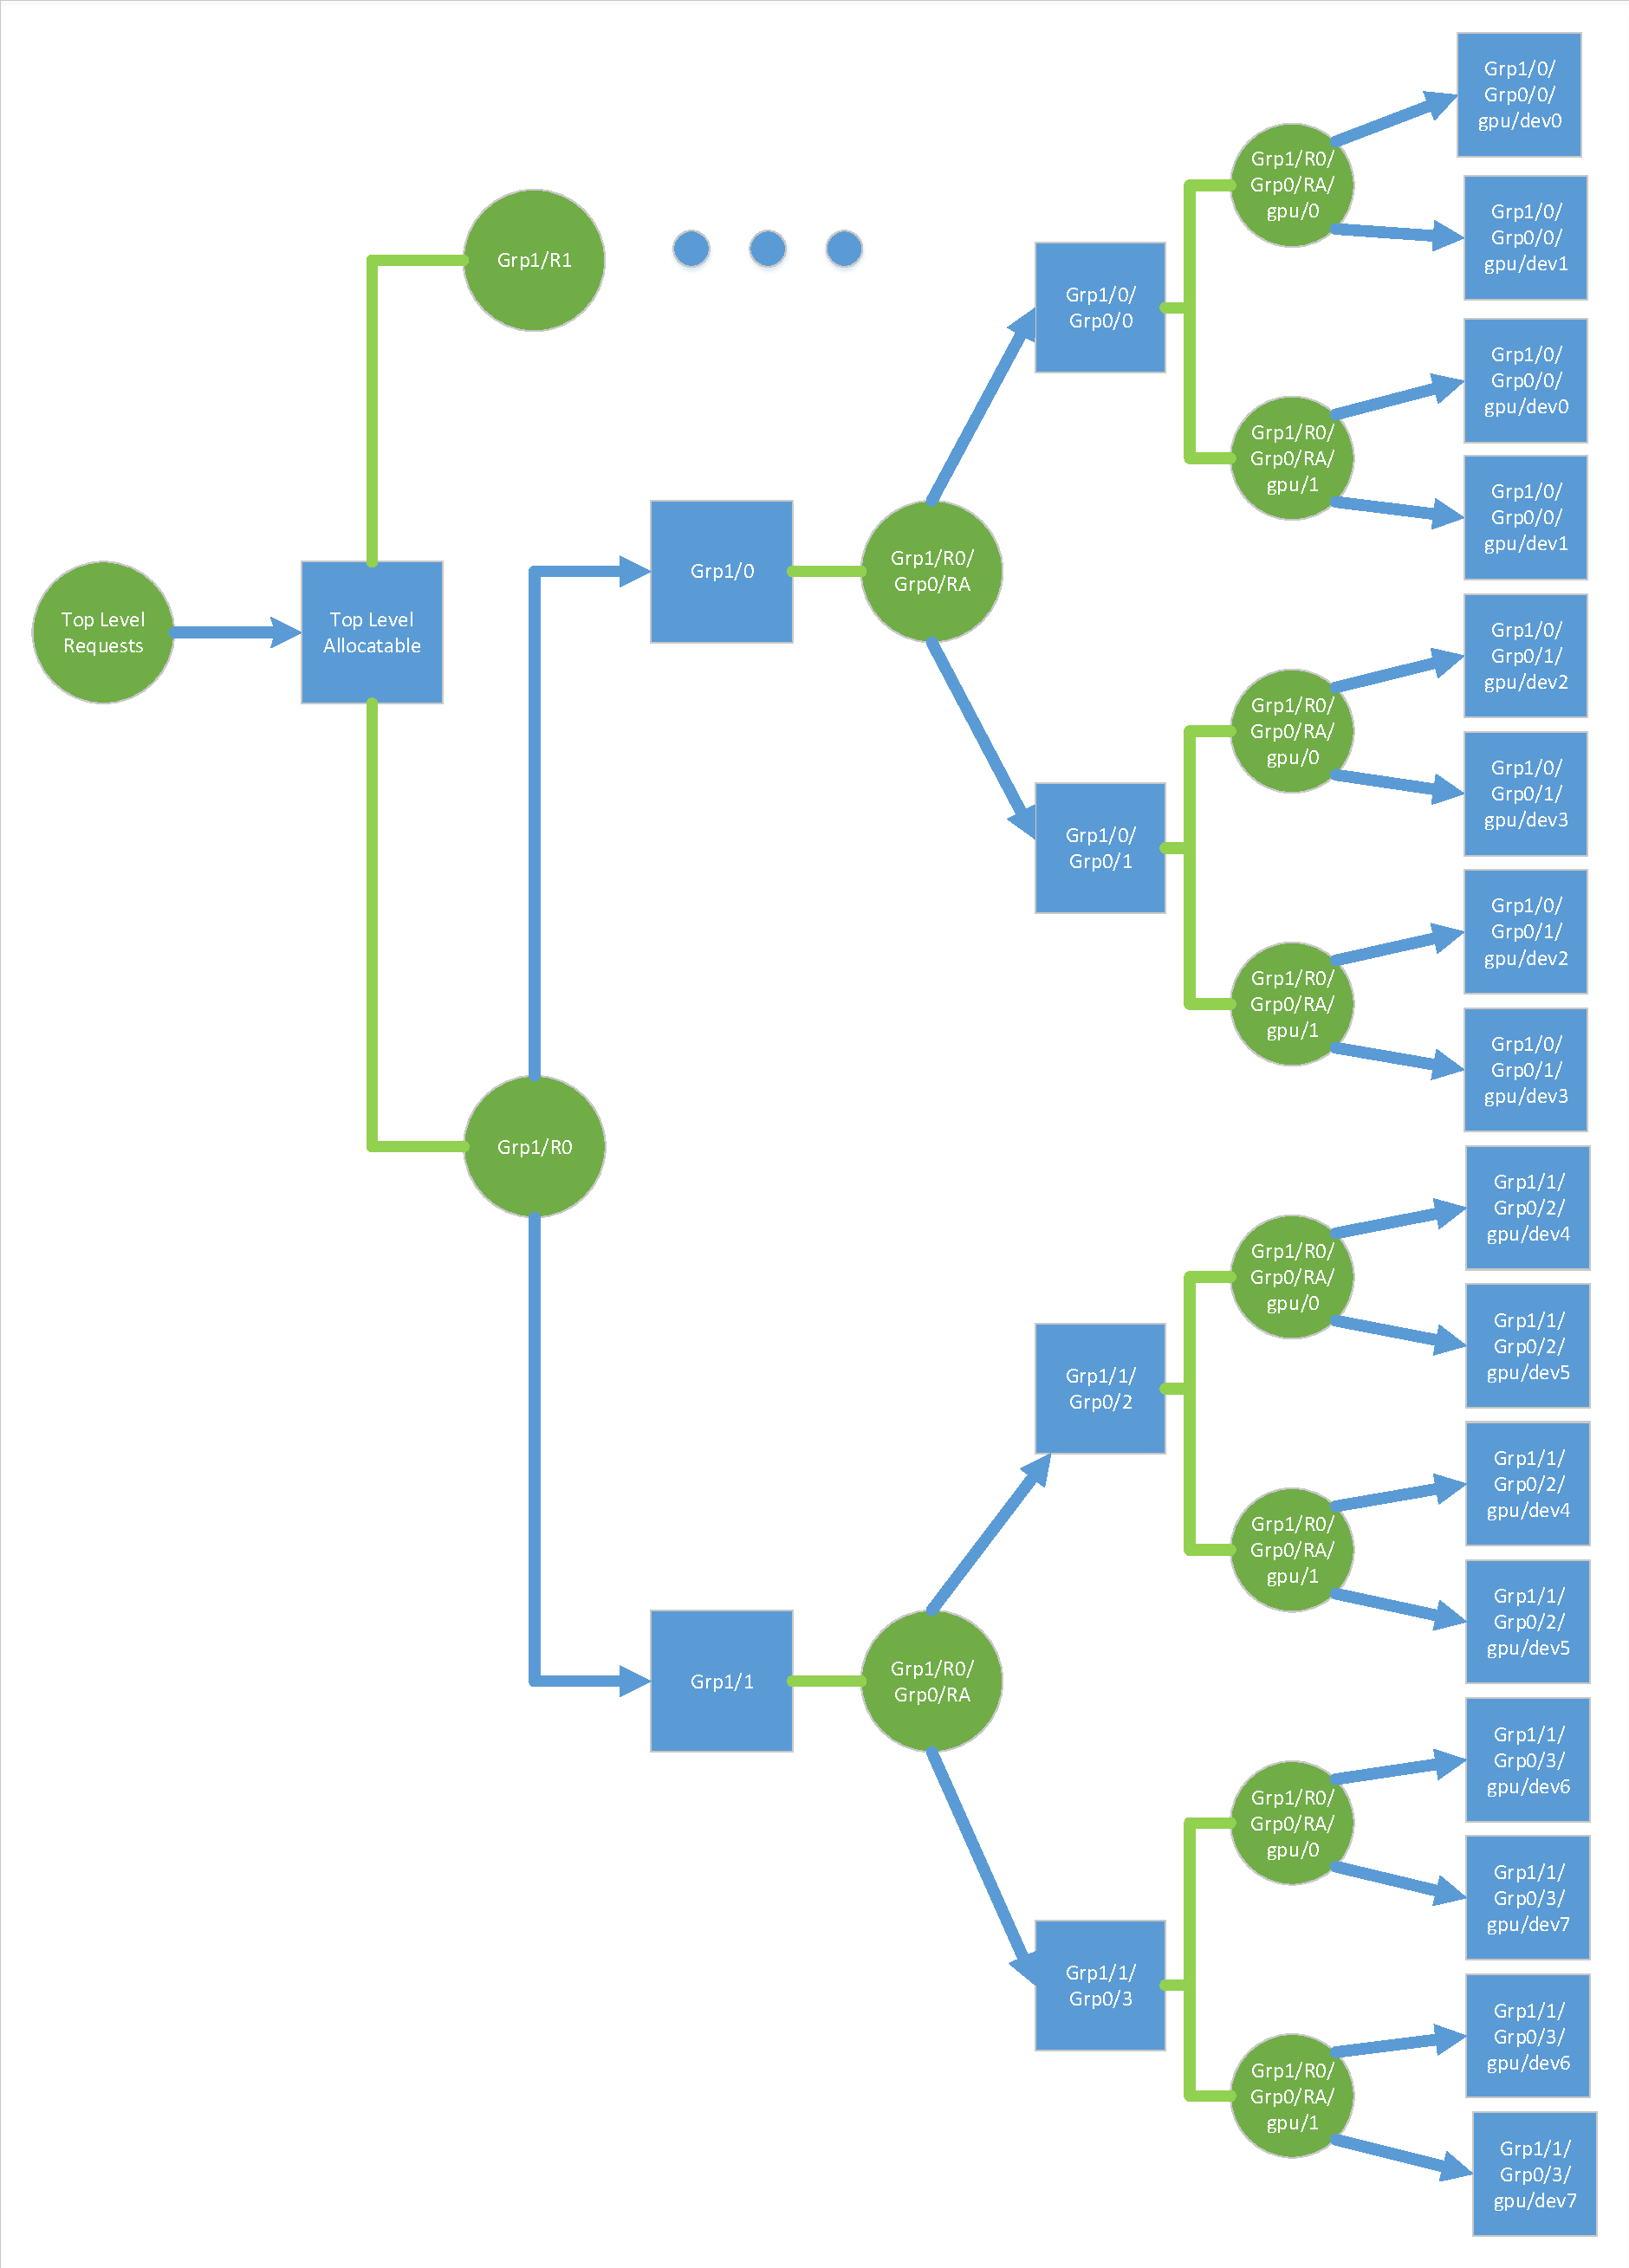
\includegraphics[width=6in]{alloc.pdf}
\caption{Figure showing the group allocators and the locations
being searched. For simplicity, ``Gpugrp'' has simply been written as ``Grp''.
The branch for \texttt{Grp1/R1} is not shown.
\label{fig:alloc}}
\end{center}  
\end{figure*}


\section{Requested Resource Translation}

For simplicity, requests may specified in the lower groups without
specifying the higher group enumeration.
For example, if we need two GPUs within the same \texttt{Gpugrp0}, we can simply
specify the request as
\ttfamily
\begin{itemize}
\item[] Gpugrp0/RA/gpu/gpu0/cards: 1
\item[] Gpugrp0/RA/gpu/gpu1/cards: 1
\end{itemize}
\normalfont
If the resources being advertised also include a \texttt{Gpugrp1}, then
the requested resources will automatically get assigned
to a unique \texttt{Gpugrp1}, a different one for each differing
\texttt{Gpugrp0}.

\end{document}


